\documentclass[12pt,a4paper,notitlepage]{article}

\usepackage[utf8]{inputenc}

\usepackage[francais]{babel}\usepackage[T1]{fontenc}
\usepackage[cyr]{aeguill}
\usepackage{lmodern}
\usepackage{color}
\usepackage{boites}
\usepackage{caption}
\usepackage{fancybox}
\usepackage{listings}
\usepackage{multicol}
\usepackage[table]{xcolor}

\usepackage[T1]{fontenc}
\usepackage[scaled]{helvet}
\renewcommand*\familydefault{\sfdefault}

%\lstset{language=bash, basicstyle=\footnotesize, frame=shadowbox, rulesepcolor=\color{gris}, captionpos=b}

  \lstset{
         basicstyle=\footnotesize\ttfamily, % Standardschrift
         %numbers=left,               % Ort der Zeilennummern
         numberstyle=\tiny,          % Stil der Zeilennummern
         %stepnumber=2,               % Abstand zwischen den Zeilennummern
         numbersep=5pt,              % Abstand der Nummern zum Text
         tabsize=2,                  % Groesse von Tabs
         extendedchars=true,         %
         breaklines=true,            % Zeilen werden Umgebrochen
         keywordstyle=\color{red},
                frame=b,         
         keywordstyle=[1]{\itshape}{//},    % Stil der Keywords
         stringstyle=\color{white}\ttfamily, % Farbe der String
         showspaces=false,           % Leerzeichen anzeigen ?
         showtabs=false,             % Tabs anzeigen ?
         xleftmargin=5pt,
         framexleftmargin=1pt,
         framexrightmargin=5pt,
         %numbers=left,
         frame=toplines,
         framextopmargin=3pt,
       %  framexleftmargin=8pt,
         numberblanklines=false,
         %morecomment=[s][marron]{/*}{*/},
         %moredelim=*[s][\color{blue}]{/*}{*/}
         %morecomment=[s][marron]{/*-}{*/}},         
         framexbottommargin=5pt,
         captionpos=b,
         %backgroundcolor=\color{lightgray},
         showstringspaces=false      % Leerzeichen in Strings anzeigen ? 
 }

\DeclareCaptionFont{white}{\color{white}}
\DeclareCaptionFormat{listing}{\colorbox[cmyk]{0.43, 0.35, 0.35,0.01}{\parbox{\textwidth}{\hspace{10pt}#1#2#3}}}
\captionsetup[lstlisting]{format=listing,labelfont=white,textfont=white, singlelinecheck=false, margin=0pt, font={bf,footnotesize}}

\definecolor{gris}{gray}{0.75}
\definecolor{bleup}{HTML}{258EE9}


%\renewcommand*\familydefault{\ttdefault} %% Only if the base font of the document is to be typewriter style
%\renewcommand{\rmdefault}{ptm}


\usepackage[
   pdfauthor={Ludovic Terrier & Arnaud Goulut},
   pdftitle={RE12 - TP5},
   ]{hyperref}
   
   
\usepackage[pdftex]{graphicx}

%\usepackage{titlesec}
%\titleformat{\section}[frame] {\normalfont} {\filright
%\footnotesize
%\enspace\textbf{\thesection}\enspace} {8pt} {\Large\bfseries\filcenter}

%% Je contrôle la taille de ma zone imprimée...
\usepackage{anysize}
%% ...en définissants les marges {gauche}{droite}{haute}{basse}
\marginsize{25mm}{15mm}{10mm}{15mm}

\begin{document}

\title{Mise en \oe uvre d'une infrastructure de ToIP}
\author{Arnaud Goulut et Ludovic Terrier}
\date{Juin 2010}
\maketitle


%\tableofcontents

\thispagestyle{empty}


 
%%%%%%%%%%%%%%%%%%%%%%%%%%%%%%%%%%% 1ère partie
\section{Etude théorique}
\subsection{SIP}
SIP est un protocole de ToIP librement utilisable via la plate-forme \textit{Asterisk}. L'intérêt d'un tel protocole en entreprise réside dans le fait que le réseau téléphonique peut être supprimé car les appels utilisent le réseau informatique.  

\paragraph{}C'est un protocole de signalisation permettant de gérer des sessions multimédia. Cette gestion passe par l'ouverture, la modification et la libération de sessions. SIP permet d'accepter un appel, indiquer une occupation ou encore identifier le mode de compression, etc. 


\paragraph{}Il permet de gérer :
\begin{enumerate}
\item la localisation des usagers,
\item la disponibilité des usagers,
\item la capacité des usagers,
\item l'établissement d'une session,
\item les sessions.
\end{enumerate}

\paragraph{}Il est normalisé par l'IETF via les RFC : 2543, 3262, 3265, etc. et est basé sur 
\begin{itemize}
\item \textit{SDP}, Session Description Portocol
\item \textit{RTSP}, Real Time Streaming Protocol 
\item \textit{RTP} (sessions de flux réel) / \textit{RTCP} (envoie régulier de paquets de contrôle par les participants à une session RTP)
\end{itemize} 

\subsubsection{Les élèments qui composent un réseau SIP}
De tels réseaux sont composés d'UA\footnote{User Agent} Serveur (qui réceptionnent les sessions), et Client (qui initialisent les sessions).
\paragraph{}Mais aussi différents types de serveurs :
\begin{itemize}
\item  Serveur d'Enregistrement (Registrar Server) : qui reçoit les inscriptions des UAs,
\item Serveur Proxy : relais mandataire utilisé entre UAs qui ne connaissent par leurs localisations respectives,
\item Serveur de localisation : contient la base de donnée des UAs.
\item Serveur de redirection : donne la localisation possible des UAs.
\end{itemize}

\subsection{messages}
SIP peut envoyer deux types de messages (textuels basés sur HTTP 1.0) :
\begin{itemize}
\item des requêtes (UAC  $\Rightarrow$ UAS)
\item des réponses
\end{itemize}

\begin{figure}[h!]
	\begin{center}
		\begin{tabular}{|c|c|c|c|}
  		 \hline
  			  \rowcolor{gris} En-tête MAC & En-tête IP & En-tête TCP ou UDP & Message SIP\\
   		 \hline
  		 \end{tabular}
		 \caption{Paquet SIP avec ses en-têtes.}
 	\end{center}
 \end{figure}
 Passons maintenant au détail d'un paquet SIP :
\begin{figure}[h!]
	\begin{center}
		\begin{tabular}{|c|c|c|}
  		 \hline
  			  \rowcolor{bleup} Type & En-tête & Corps\\
   		 \hline
		 	INVITE & VIA   &    \\
			REGISTER & FROM & Description de  \\
			ACK &  TO &  la session par \\
			BYE &   CALL-ID  &   le protocole SDP   \\
			CANCEL &   CSEQ &  \\
		 \hline
  		 \end{tabular} 
		 \caption{Détail d'un paquet SIP.}
 	\end{center}
 \end{figure}
\paragraph{} Revenons sur le paramètre \textit{Cseq} contenu dans l'en-tête, celui-ci est un indentifiant d'échanges liant les requêtes aux réponses. Il est incrémenté à chaque nouvelle requête.

\section{Architecture utilisée}
\subsection{Configuration réseau}
\begin{figure}[!h]
\begin{center}
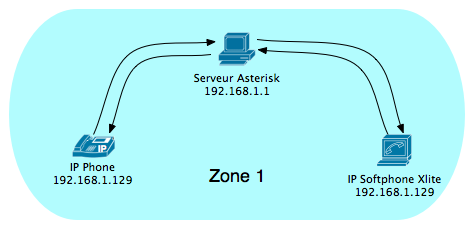
\includegraphics[height=5cm]{structure_reseau}
\caption{Structure du réseau}
\label{fig:da}
\end{center}
\end{figure}

\subsection{Configuration téléphone}
\clearpage
\section{Fichiers de configuration SIP}
\subsection{sip.conf}

\begin{lstlisting}[title=sip.conf v1]
[user1]
username=user1
type=friend
context=locale ;outgoing
port=5060
quality=200
;secret=blah
nat=no
host=dynamic
canreinvite=yes

[user2]
username=user2
type=friend
context=locale ;outgoing
port=5060
quality=200
;secret=blah
nat=no
host=dynamic
canreinvite=yes
\end{lstlisting}

\subsection{extensions.conf}

\begin{lstlisting}[title=Extensions.conf v1]
[locale]
exten => 101,1,Wait(1)
exten => 101,2,Dial(SIP/user1)
exten => 101,3,Hangup

exten => 102,1,Wait(1)
exten => 102,2,Dial(SIP/user2)
exten => 102,3,Hangup
\end{lstlisting}

\clearpage
\section{IAX} 
\subsection{Pourquoi?}
A ce stade nous sommes en mesure de passer des appels entre divers téléphones situés sur le même réseau via le même serveur Asterisk. Or, parfois en entreprise, dans le cas de postes géographiquement séparés il peut être intéressant de pouvoir appeler des téléphones sur d'autres réseaux et utilisant un autre serveur de ToIP. Ceci est permit par le protocole IAX\footnote{Inter-Asterisk eXchange}. Pour les besoins du TP nous l'avons implémenté afin de pouvoir échanger des appels téléphoniques entre tous les groupes.

\paragraph{}Voici le schéma décrivant l'infrastructure du réseau que nous désirons obtenir :

\begin{figure}[!h]
\begin{center}
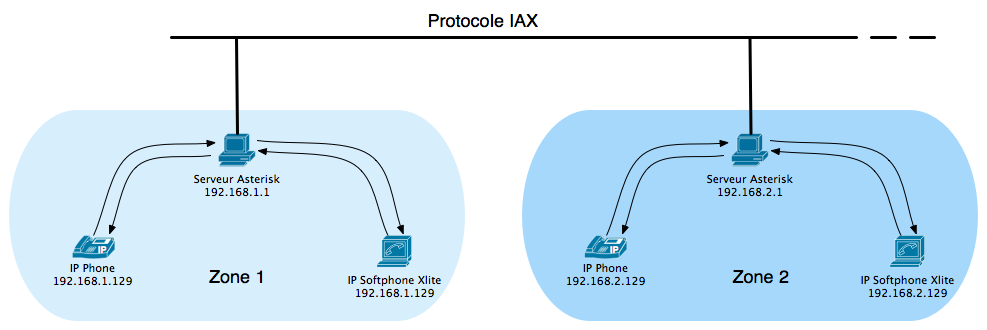
\includegraphics[height=5cm]{structure_reseau_IAX}
\caption{Structure du réseau}
\label{fig:da}
\end{center}
\end{figure}

\subsection{Fichier IAX.conf}

Tout d’abord, nous ajoutons les autres serveurs Asterisk dans le fichier \\
\texttt{/etc/asterisk/iax.conf} :

\begin{lstlisting}[title=Fichier IAX.conf]
[serveur4]
type=friend
username=serveur4
host=192.168.4.129
mask=255.255.255.128
secret=123456
port=4569
context=locale
auth=md5
trunk=yes

[serveur5]
type=friend
username=serveur3
host=192.168.5.1
mask=255.255.255.128
secret=123456
port=4569
context=locale
auth=md5
trunk=yes

[serveur2]
type=friend
username=serveur2
host=192.168.2.1
mask=255.255.255.128
secret=123456
port=4569
context=locale
auth=md5
trunk=yes
\end{lstlisting}
Nous avons ajouté ici, les serveurs \textit{4}, \textit{5} et \textit{2}. Nous avons définit le \textbf{type friend}, en effet dans ce cas les utilisateurs de notre réseau peuvent \textit{appeler} et être \textit{appelés}. Nous indiquons ensuite le nom du serveur via la commande \textbf{username} ainsi que son adresse IP avec le masque de sous réseau ainsi que le port. Vient ensuite le mot de passe utilisé pour s'authentifier sur le serveur distant via md5 (le champ \textbf{auth}). Enfin, \textbf{trunk=yes} permet de signifier au serveur qu'il peut utiliser les timeslots qui lui sont attribués pour plusieurs appels.

\section{Fichiers de traces}
\subsection{Message INVITE (en détail)}
Un paquet d'INVITE SIP est composé de deux parties, un \textit{HEADER} et un  \textit{BODY}. C'est le détail de ces deux éléments que nous allons voir ici. 

\paragraph{}Pour ce faire nous avons émit un appel entre un hardphone (IP 192.168.3.129) vers un softphone X-lite (IP 192.168.3.3). Nous avons capturé à l'aide de Wireshark l'ensemble des échanges depuis le serveur. Ainsi nous pouvons vous proposer ici le contenu du paquet INVITE capturé entre l'émetteur et le serveur Asterisk :
\subsubsection{HEADER}
\begin{lstlisting}[title=Contenu du HEADER d'un paquet INVITE de SIP]
 Via: SIP/2.0/UDP 192.168.3.129:5060;rport;branch=z9hG4bK31769CB150326F07D6EF3F1EE6061B5B
        From: user1 <sip:user1@192.168.3.1>;tag=1600664632
        To: <sip:102@192.168.3.1>
        Contact: <sip:user1@192.168.3.129:5060>
        Call-ID: 706088E9-6905-7FA9-B9A8-F002AC583FF6@192.168.3.129
        CSeq: 43045 INVITE
        Max-Forwards: 70
        Content-Type: application/sdp
        User-Agent: X-Lite release 1105d
        Content-Length: 312
\end{lstlisting}

\subsubsection{BODY}
\begin{lstlisting}[title=Contenu du BODY d'un paquet INVITE de SIP]

Session Description Protocol
            Session Description Protocol Version (v): 0
            Owner/Creator, Session Id (o): user1 4092070068 4092070070 IN IP4 192.168.3.129
            Session Name (s): X-Lite
            Connection Information (c): IN IP4 192.168.3.129
            Time Description, active time (t): 0 0
            Media Description, name and address (m): audio 8000 RTP/AVP 0 8 3 98 97 101
            Media Attribute (a): rtpmap:0 pcmu/8000
            Media Attribute (a): rtpmap:8 pcma/8000
            Media Attribute (a): rtpmap:3 gsm/8000
            Media Attribute (a): rtpmap:98 iLBC/8000
            Media Attribute (a): rtpmap:97 speex/8000
            Media Attribute (a): rtpmap:101 telephone-event/8000
            Media Attribute (a): fmtp:101 0-15
            Media Attribute (a): sendrecv
\end{lstlisting}

\subsection{Message BYE} 
Voyons ici le contenu d'un paquet BYE émis par l'UA\footnote{User Agent} qui était à l'initiative de l'appel.

\begin{lstlisting}[title=Contenu d'un paquet BYE]
Session Initiation Protocol
    Request-Line: BYE sip:102@192.168.3.1 SIP/2.0
    Message Header
        Via: SIP/2.0/UDP 192.168.3.129:5060;rport;branch=z9hG4bK345EE39524AA335D955FEC4B5AC9A503
        From: user1 <sip:user1@192.168.3.1>;tag=1600664632
        To: <sip:102@192.168.3.1>;tag=as16bb0d2a
        Contact: <sip:user1@192.168.3.129:5060>
        Call-ID: 706088E9-6905-7FA9-B9A8-F002AC583FF6@192.168.3.129
        CSeq: 43046 BYE
        Max-Forwards: 70
        User-Agent: X-Lite release 1105d
        Content-Length: 0
\end{lstlisting}







\end{document}